In the finite volume method (FVM), the spatial domain is discretized into a set of volumes.\footnote{In 1D, the ``volumes'' are simply line segments.}
In the FVM, unlike the finite element method, information is stored at the center of the volume.
The goal has thus been changed from solving directly for $u$ and now for $\bar{u}$, which is defined as:
\begin{equation}
	\label{eq:u-bar}
	\begin{split}
		\bar{u}&=\frac{\int_{\Omega_V} u \dd \Omega_V }{\int_{\Omega_V}\dd \Omega_V }\\
		&=\frac{1}{V}\int_{\Omega_V} u \dd \Omega_V
	\end{split}
\end{equation}
where $\Omega_V$ defines the spatial domain of a single arbitrary volume in the global domain, $\Omega$.
\Cref{fig:domain and subdomain} provides a graphical representation.
The second line in \cref{eq:u-bar} defines $V\equiv\int_{\Omega_V}\dd \Omega_V $, the cell volume, and simplifies the first line.
Notice that \cref{eq:u-bar} defines the \textit{volume-averaged} value of $u$ in the cell.
The implicit assumption is that $u$ varies only slightly in the volume, and this assumption is valid with a sufficiently small spatial discretization.
\begin{figure}
	\centering
	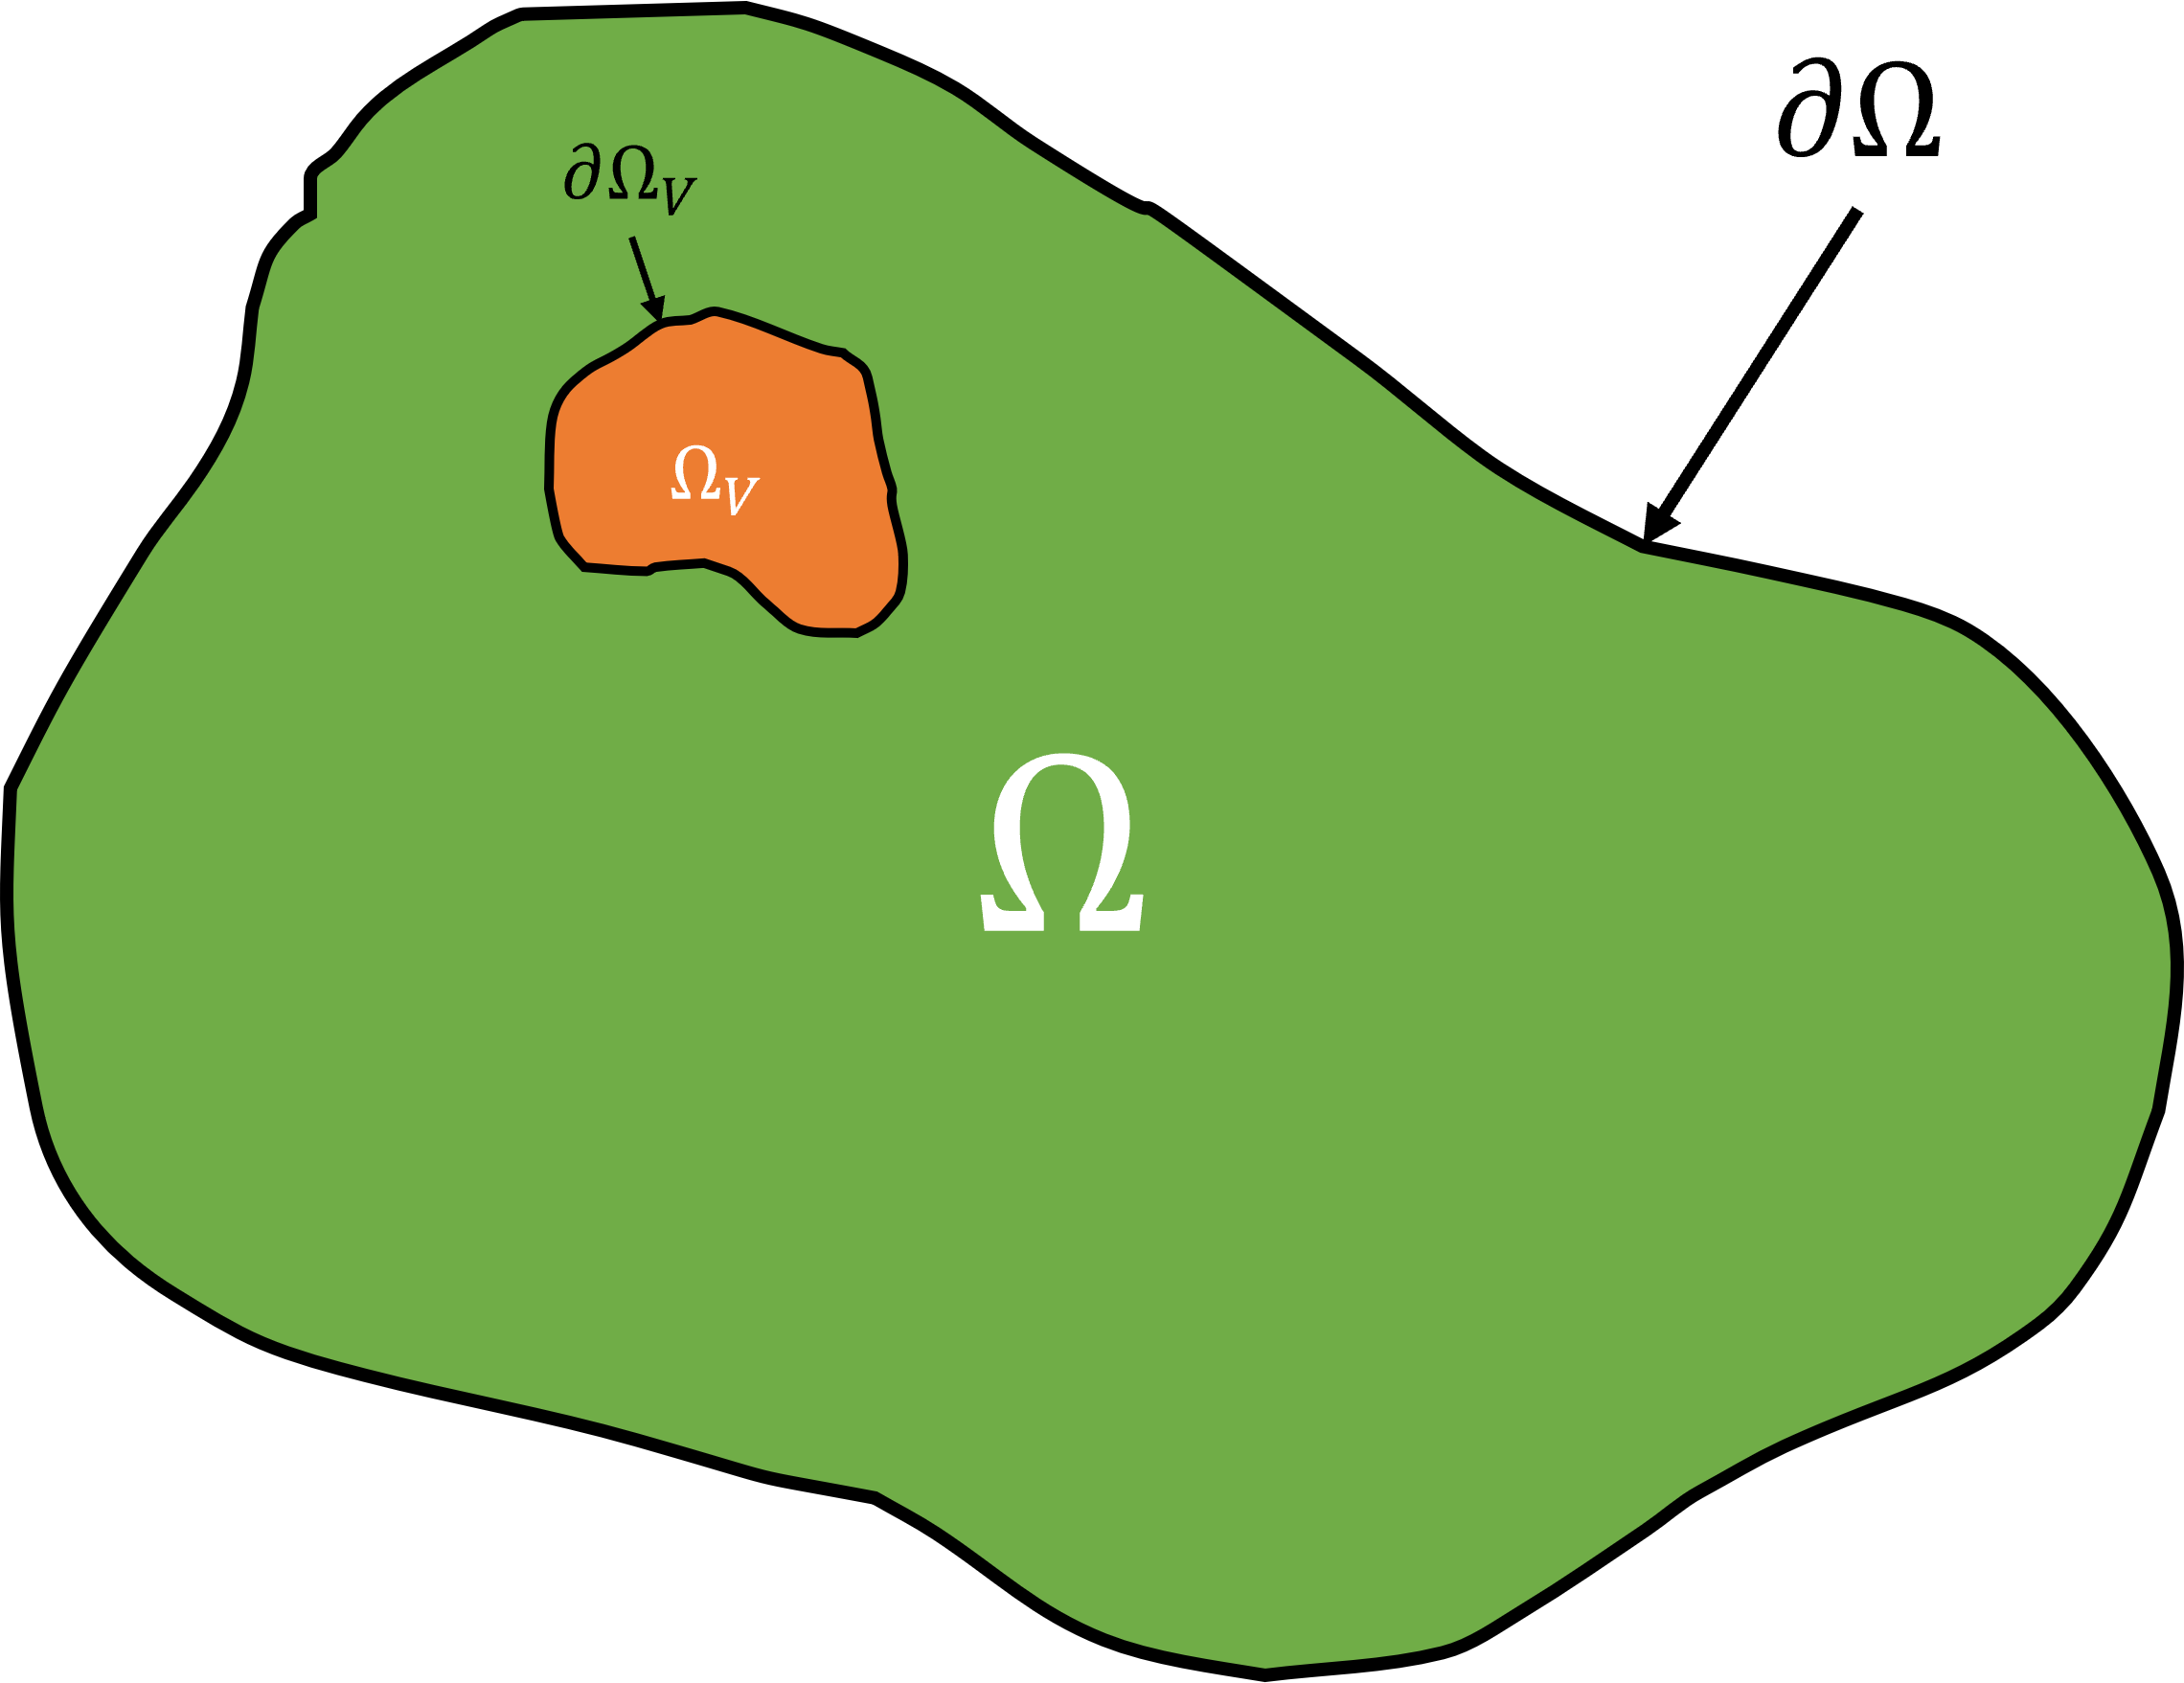
\includegraphics[width=0.6\textwidth]{figures/domain_subdomain}
	\caption{Arbitrary domain and volume subdomain.}
	\label{fig:domain and subdomain}
\end{figure}
Substituting \cref{eq:u-bar} into \cref{eq:burgers-equation} gives the following:
\begin{equation}
	\label{eq:u-averaged-burgers}
	\pdv{\bar{u}}{t} + \bar{u}\pdv{\bar{u}}{x} = \nu \pdv[2]{\bar{u}}{x}
\end{equation}

\Cref{eq:u-bar} has only integrated the function over a discretized volume, not the entire domain, giving the average value of the function within the volume.
Integrating over the entire spatial domain gives\footnote{This is the main step of the FVM, and it carries with it important properties of conservation. Therefore, for applications such as fluid mechanics, properties such as mass are guaranteed to be conserved, leading to a physically-representative solution.}:
\begin{equation}
	\label{eq:finite-volume-aribitrary-domain}
	\int_{\Omega}\bar{u}_t \dd \Omega + \int_{\Omega}  \bar{u}\bar{u}_x\dd \Omega = \int_{\Omega}\nu \bar{u}_{xx}\dd \Omega
\end{equation}
\Cref{eq:finite-volume-aribitrary-domain} was written with a more general notation where $\Omega$ is some arbitrary domain.
When the domain is in 1D and has been discretized into $m$ finite volumes, the system would instead be written as:
\begin{equation}
	\label{eq:finite-volume-implemented}
	\sum_{i=0}^{m-1} \left[  \int_{i-1/2}^{i+1/2} \bar{u}_t \dd \left(\Omega_V\right)_i+\int_{i-1/2}^{i+1/2} \bar{u}\bar{u}_x \dd \left(\Omega_V\right)_i \right]=\sum_{i=0}^{m-1}\left[ \int_{i-1/2}^{i+1/2} \nu \bar{u}_{xx}\dd \left(\Omega_V\right)_i \right]
\end{equation}
The index $i$ represents the center of the volume, so $i\pm 1/2$ is boundary of the volume.
Applying the divergence theorem\footnote{This step may seem overcomplicated, but it is ubiquitous in FVM methods, particularly for more complicated equations such as the Navier-Stokes. This step is introduced this way to ensure the reader understands its importance, trivial as it may be for a 1D case.}, which is defined as~\autocite{CalculusIIIDivergence}:
\begin{equation}
	\label{eq:divergence-thm}
	\iiint_{\Omega}\div \vec{f}\dd V = \oiint_{\partial \Omega} \vec{f}\cdot \hat{n}\dd S
\end{equation}
where $\vec{f}$ is some vector-valued function, $\Omega$ is an arbitrary domain, and $\partial \Omega$ is the domain's boundary, gives the following:
\begin{equation}
	\label{eq:finite-volume-solution}
	\bar{u}_t \Delta x +\left( \left( \frac{\bar{u}^2}{2}\right)_{i+1/2}-\left( \frac{\bar{u}^2}{2}\right)_{i-1/2} \right)=\nu \left( \pdv{\bar{u}}{x}\eval_{i+1/2}-\pdv{\bar{u}}{x}\eval_{i-1/2} \right)
\end{equation}
It is noted that a shortcut has been taken in the first integral:
\begin{equation*}
	\begin{split}
		\int_{i-1/2}^{i+1/2} \bar{u}_t \dd \left(\Omega_V\right)_i&=\bar{u}_t\int_{i-1/2}^{i+1/2} \dd \left(\Omega_V\right)_i\\
		&=\bar{u}_{t}V_i
	\end{split}
\end{equation*}
where $V_i$ is the volume of $i$\textsuperscript{th} volume.
$V_i$ in 1D is simply the length along the domain.
More on this is discussed in \cref{sec:boundary-conditions-and-implementation}, but for now, assume the domain has been discretized into equally-spaced, 1D volumes of length $\Delta x$.

To solve \cref{eq:finite-volume-solution}, both the functional values and the derivatives at the boundaries must be known.
As discussed with \cref{eq:u-bar}, only the average value of the cell is known.
Necessarily, the solution is assumed and often expected to be discontinuous on the volume boundaries.\footnote{A perfectly continuous case would imply a steady solution with no spatial variation.}

Approximation techniques are now used to describe these values.
The derivatives at the boundaries can be approximated in a straightforward manner with finite differencing.
To derive the stencil, one expands $\pdv{u}{x}\eval_{i\pm 1/2}=u_x\eval_{i\pm 1/2}$ using two Taylor series~\autocite{yewNumericalDifferentiationFinite2011a}:
\begin{subequations}
	\begin{equation}
		\label{eq:first-taylor-expansion}
		u_x\eval_{i+1/2}=u_x\eval_i+\left( \frac{\Delta x}{2} \right)u_{xx}\eval_{i}+\frac{1}{2!}\left( \frac{\Delta x}{2} \right)^2 u_{xxx}\eval_i+\order{\left( {\Delta x} \right)^3}
	\end{equation}
	\begin{equation}
		\label{eq:second-taylor-expansion}
		u_x\eval_{i-1/2}=u_x\eval_i-\left( \frac{\Delta x}{2} \right)u_{xx}\eval_{i}+\frac{1}{2!}\left( \frac{\Delta x}{2} \right)^2 u_{xxx}\eval_i+\order{\left( {\Delta x} \right)^3}
	\end{equation}
\end{subequations}
The subscript $x$ in $u_x$ indicates a derivative with respect to $x$, so $u_{xx}=\pdv[2]{u}{x}$ and $u_{xxx}=\pdv[3]{u}{x}$.
The symbol $\order{}$ is known as ``big-O'' notation, and it describes the dominant term in an infinite series.
Because $\left( \Delta x \right)^3>\left( \Delta x \right)^4>\ldots$, it is said that the error terms increase on an ``order of $\left( \Delta x \right)^3$.''
Subtracting \cref{eq:second-taylor-expansion} from \cref{eq:first-taylor-expansion} gives the following:
\begin{equation}
	\label{eq:flux-difference-result}
	u_x\eval_{i+1/2}-u_x\eval_{i-1/2}=\Delta x u_{xx}\eval_i+\order{ (\Delta x)^3 }
\end{equation}
An approximation for $u_{xx}\eval_i$ must now be found.
Fortunately, this process is simple because resources such as~\autocite{yewNumericalDifferentiationFinite2011a} have already derived high-order methods, such as two-point central differencing, for finding the value of the derivative at a volume center.
\begin{equation}
	\label{eq:spatial-finite-difference-2nd-derivative}
	u_{xx}\eval_i=\frac{u_{i+1}-2u_i+u_{i-1}}{\left( \Delta x \right)^2}+\order{\left(\Delta x \right)^2}
\end{equation}
\Cref{eq:spatial-finite-difference-2nd-derivative}, finally arrives at the following:
\begin{equation}
	\label{eq:wall-derivative-approx}
	u_x\eval_{i+1/2}-u_x\eval_{i-1/2}=\frac{u_{i+1}-2u_i+u_{i-1}}{\Delta x}+\order{ (\Delta x)^3}
\end{equation}
The nonlinear terms in \cref{eq:finite-volume-solution}, however, prove to be significantly more difficult.
Defining $f\equiv\frac{u^2}{2}$ and rewriting \cref{eq:finite-volume-solution} gives the following:
\begin{equation}
	\label{eq:burgers-equation-with-fluxes}
	u_t + \frac{1}{\Delta x}\left( f_{i+1/2}-f_{i-1/2} \right)=\frac{1}{\Delta x}\nu \left( \pdv{\bar{u}}{x}\eval_{i+1/2}-\pdv{\bar{u}}{x}\eval_{i-1/2} \right)
\end{equation}
Substituting \cref{eq:wall-derivative-approx} to the right hand side gives:
\begin{equation}
	\label{eq:burgers-eq-central-diff}
	u_t + \frac{1}{\Delta x}\left( f_{i+1/2}-f_{i-1/2} \right)=\frac{\nu }{\left( \Delta x \right)^2}\left( u_{i+1}-2u_1+u_{i-1} \right)+\order{\left( \Delta x\right)^2 }
\end{equation}
The terms $f_{i\pm 1/2}$ are known as \textit{numerical flux} terms and are defining characteristics of advection equations.
These terms will be discussed in the next section.
Additionally, the bar seen above the function terms $u$ is omitted for brevity, although all solutions discussed are volume-averaged values defined by \cref{eq:u-bar}.

\Cref{eq:burgers-eq-central-diff} has only one approximation, and that approximation has an error that scales quadratically with the spatial step size.
In order to not waste efforts in achieving second-order accuracy, time and flux discretizations that are at least second-order accurate must be similarly chosen.